\subsection{Electrophysiology of Speech Perception}
  
EEG distribution coding is a proposed new method that interprets the
pre-categorical electrical evoked potentials of untrained listeners
(measured by an electro-encephalograph or EEG) as a posterior
probability distribution over the phone set of the utterance language
(Fig.~\ref{fig:eeg_paradigm}).  Transcribers, in this scenario, first
listen to speech in their native language, and their EEG responses are
recorded.  From their responses to English speech, an English-language
EEG phone recognizer is trained, using methods based
on~\cite{Liberto15}.  In order to estimate the misperception
probabilities $\rho(\psi|\phi)$, then, non-native syllables are played
to the same listeners.  For each non-native phone $\phi$, the
classifier outputs are interpreted as an estimate of $\rho(\psi|\phi)$
for all $\phi\in\mathbb{\Phi}$, the native phone inventory.

\begin{figure}
  \centerline{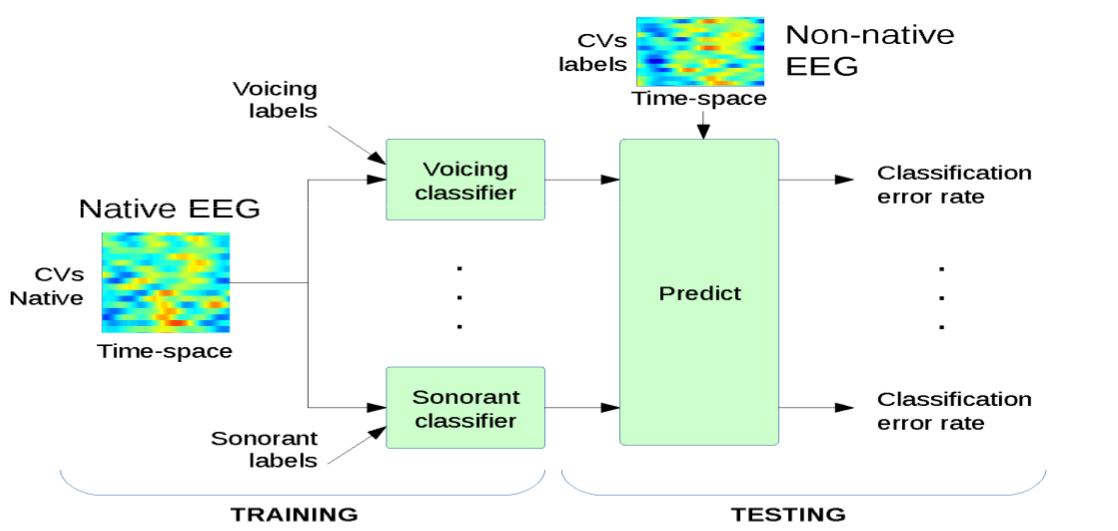
\includegraphics[width=4in]{../figs/diliberto_paradigm.png}}
  \caption{EEG responses are recorded while listeners hear speech in
    their native language.  For each listener, a bank of distinctive
    feature classifiers are trained.  The same listeners then hear
    speech in a non-native language, and the same classifiers are
    applied, estimating a listener-language transcription of the
    non-native speech.}
  \label{fig:eeg_paradigm}
\end{figure}

